\part{Nicht in der endgültigen Arbeit}

\chapter{Seitenränder}
\url{http://www.latex-project.org/guides/lb2-ch4.pdf}  aus "`Der \LaTeX-Begleiter"' (978-3827370440 -- \url{http://www.amazon.de/LaTeX-Begleiter-Michel-Goossens/dp/3827370442})

\the\oddsidemargin \\
\the\evensidemargin \\
\the\hoffset \\
\the\footskip


\chapter{Sonstiges}

\todo{Dieses Kapitel dient nur dazu unsortierte Textabschnitte aufzunehmen. Es wird nicht Teil der Arbeit.}

\cite{brandstaedt1999graph}
\cite{Cardoso2011}
\cite{ClWidthSOL}
\rule{\linewidth}{1pt}
\clearpage

\section{Pflichtkanten}
\todo{Eventuell andere Übersetzung oder engl Begriff}

Für einen Graphen ist ein dim nicht immer eindeutig. Es kann mehrere mögliche Varianten in einem Graphen geben. Es ist jedoch so, dass in einigen Fällen auch bei verschiedenen dims, einzelne Kanten zwingend in jedem dim des Graphen enthalten sein müssen.

\begin{mydef}[Pflichtkante]
Gegeben sei ein Graph $G=(V,E)$. Eine Kante $m\in E$ ist eine \emph{Pflichtkante} (engl.: mandatory edge), wenn für alle dims $M$ von $G$ gilt: $m\in M$.
\end{mydef}

In einem Diamond $D$ ist beispielsweise die mittlere Kante eine Pflichtkante. Wählt man eine andere Kante (am Rand), so ist die gegenüberliegende Kante zu nahe an der gewählten um zum dim zu gehören. Wenn $D$ Teilgraph eines größeren Graphen ist, bliebe noch die Möglichkeit, dass die gegenüberliegende Kante mit einer Kante des dims verbunden ist. Auch das ist nicht möglich, da diese Kanten ebenfalls zu nahe wären.

\todo{alternativ über Knotenklassen beschrieben, oder vorher zeigen, dass in einem Dreieck eine Kante enthalten sein muss.}

\begin{figure}[htb]
\centering
\hspace*{\fill}
\subfloat[Diamond]{\begin{tikzpicture}
  [thick,
   normalN/.style={circle,draw,minimum size=0.25cm,inner sep=0pt,fill=white},
   colE/.style={draw,-,line width=0.075cm}
  ]

  \foreach \x/\y in {0/a,90/b,180/c,-90/d} {
     \node[normalN] (\y) at (\x:0.75cm) {};
  }

  \node (e) at (0:1.5cm) {};
  
    \begin{pgfonlayer}{background}
        \draw [colE,blue] (c.center) -- (b.center);
        
        \draw [colE,darkgreen] (a.center) -- (b.center);
        \draw [colE,darkgreen] (a.center) -- (c.center);
        \draw [colE,darkgreen] (c.center) -- (d.center);
        
        \draw [colE,red] (a.center) -- (d.center);

        \draw [colE,red, dashed] (a.center) -- (e.center);
    \end{pgfonlayer}
   
 
\end{tikzpicture}}
\hspace*{\fill}
\subfloat[Gem]{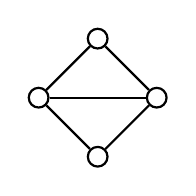
\begin{tikzpicture}
  [thick,
   normalN/.style={circle,draw,minimum size=0.25cm,inner sep=0pt,fill=white}
  ]

  \foreach \x/\y in {0/a,90/b,180/c,-90/d} {
     \node[normalN] (\y) at (\x:0.75cm) {};
  }
  
  \foreach \x/\y in {a/b,b/c,c/d,d/a,a/c} {
      \draw (\x) -- (\y);
  }

 
\end{tikzpicture}}
\hspace*{\fill}
\caption{TODO}
\label{pic:bsp_mandEdge}
\end{figure}


\rule{\linewidth}{1pt}
\clearpage

\begin{Lemma}\label{lem:simplClique}Es sei $H$ ein Hypergraph mit $\mL=L(H)$ und einem dim $M$. Für jede Clique $K$ in $\mL$ mit einem simplizialen Knoten $s$ gilt:
\[\exists!\,v\in K:v\in M\]
\end{Lemma}

\begin{Proof}
Angenommen es gehört kein Knoten aus $K$ zu $M$. Dann ist $s$ nicht mit einem Knoten aus $M$ benachbart. Somit ist $M$ auch kein dim von $H$. Folglich gibt es einen Knoten $v\in K$.

Offensichtlich ist es genau ein Knoten, da in einer Clique von $\mL$ höchstens ein Knoten zu $M$ gehören kann. Andernfalls wären zwei Knoten aus $M$ miteinander benachbart.
\qed
\end{Proof}

\rule{\linewidth}{1pt}
\clearpage

\begin{Lemma}
Es sei $H$ ein Hypergraph und $\mL$ dessen Linegraph. Des weiteren sei $N_B(v)=\{b\ |\ b\in N(v)\wedge b\text{ ist Blatt}\}$ die Menge der benachbarten Blätter eines Knotens $v$ aus $\mL$.

Wenn $\left|N_B(v)\right|\geq2$, dann ist $v$ eine Pflichtkante in $H$.
\end{Lemma}

Ergibt sich aus Lemma \ref{lem:simplClique}

\rule{\linewidth}{1pt}
\clearpage

\section{Bereinigung von Zwillingen}

\begin{mydef}[Nachbarschaft eines Knotens]
    Gegeben sei ein Graph $G=(V,E)$. Die \emph{offene} Nachbarschaft $N(v)$ bzw. die \emph{abgeschlossene} Nachbarschaft $N[v]$ von $v$ seien dann wie folgt definiert:
    \begin{align*}
        N(v)&:=\{u\ |\ uv \in E\} \\
        N[v]&:=N(v) \cup \{v\}
    \end{align*}
\end{mydef}

\begin{mydef}[Zwillinge]
    In einem Graphen werden zwei Knoten $u$ und $v$ ($u\neq v$) als (echte) Zwillinge bezeichnet (engl. true twins), wenn $N[u]=N[v]$.
\end{mydef}

Bei Zwillingen gilt es zu beachten, dass es sich um eine abgeschlossene Nachbarschaft handelt. Somit müssen zwei Knoten $u$ und $v$ nicht nur die selben Nachbarn haben, sondern auch selbst benachbart sein. Es muss also eine Kante $uv$ vorhanden sein.

\subsection{Die Funktion $t()$}
\todo{Funktion besser beschreiben}
Gegeben ein Graph $G=(V,E)$.
\begin{description}
\item[Schritt 1] Für alle $v\in V$: Wenn $v$ einen Zwilling $u$ besitzt, dann $V:=V\,\backslash\,\{v\}$

\item[Stopp]
\end{description}

Der so erzeugte Graph $t(G)$ sei der um Zwillinge bereinigte Graph von $G$.

\begin{Lemma}
    Ein Graph $G$ hat ein vDim genau dann, wenn $t(G)$ ein vDim hat.
\end{Lemma}
\todo{Eventuell Abb. für Beweis}
\begin{Proof}
	Es seien $u$ und $v$ Zwillinge in $G$, wobei $u$ kein Knoten in $t(G)$ ist.
	
    \prR $G$ habe ein vDim $D$. Es gibt nun zwei mögliche Fälle:
    \begin{enumerate}
        \item $u$ gehört nicht zu $D$. Durch das entfernen von $u$ bleibt $D$ ein gültiges vDim in $t(G)$.
        \item $u$ gehört zu $D$. In diesem Fall ist $(D\,\backslash\,\{u\})\cup\{v\}$ ein gültiges vDim in $t(G)$. Da $u$ und $v$ Zwillinge sind, werden nun alle Knoten durch $v$ gematcht, die vorher durch $u$ gematcht wurden.
    \end{enumerate}

    \prL $t(G)$ habe ein vDim $D$. Es sei $d$ der Knoten, durch den $v$ gematcht wird. $d$ matcht aufgrund der identischen Nachbarschaft auch $u$ in $G$. Somit ist $D$ auch ein gültiges vDim in $G$.
    \qed
\end{Proof}

Somit kann o. B. d. A. angenommen werden, dass ein Linegraph, in dem ein vDim gesucht wird, keine Zwillinge mehr besitzt.

\rule{\linewidth}{1pt}
\clearpage


\section{Vereinfachung eines Hypergraphen}

\todo{Darstellung für Algorithmen}

Es sein $E(v):=\{e\in \mE \ |\ v\in e\}$ die Menge der Hyperkanten, in denen der Knoten $v$ ist.

\subsection{Die Funktion $m(H)$}
\todo{eventuell besser formulieren}
Gegeben ein Hypergraph $H=(V,\mE)$.
\begin{description}
\item[Schritt 1] Für alle $v\in V$: Wenn $E(v)=\{e\}$ und $|e|>1$, dann $H:=H\backslash\{v\}$.

\item[Schritt 2] Für alle $v\in V$: Wenn $\exists\,u:u\neq v$ und $E(u)=E(v)$, dann $H:=H\backslash\{v\}$.

\item[Stopp]
\end{description}

Der so erzeugte Graph sei $m(H)$.

\subsection{Beibehalten relevanter Eigenschaften}
\subsubsection{Beibehalten der Dominating Induced Matchings}
\begin{Theorem}
$H$ hat dim $\Leftrightarrow$ $m(H)$ hat dim.
\end{Theorem}

\begin{Proof}
Es werden weder Kanten entfernt, noch hinzugefügt. Auch die Nachbarschaft der Kanten wird nicht verändert. \qed
\end{Proof}

\subsubsection{Beibehalten der Chordalität}
\todo{Gibts das Wort Chordalität? -- Eventuell andere Formulierung}

\begin{Lemma}\label{lem:JedeKanteAndereHyperkante}
Es sei $C$ ein $C_k$ ($k\geq 4$) und induzierter Teilgraph von $2Sec(H)$, dann gilt: Jede Kante aus $C$ gehört zu einer anderen Hyperkante.
\end{Lemma}

\begin{Proof}
Angenommen zwei Kanten $e_1=u_1v_1$ und $e_2=u_2v_2$ von $C$ mit $u_1\neq v_2$ gehören zur gleichen Hyperkante von $H$. Dann ist $u_1v_2$ eine Kante in $2Sec(H)$. Somit ist $C$ kein induzierter Teilgraph von $2Sec(H)$. \qed
\end{Proof}

\begin{Theorem}\label{theo:ChordalM}
$2Sec(H)$ ist chordal $\Leftrightarrow$ $2Sec(m(H))$ ist chordal.
\end{Theorem}

\todo{Alternativ für $\Rightarrow$ zeigen, dass: $\forall\,u,v \in m(H)$ gilt: $uv\in 2Sec(H) \Leftrightarrow uv\in 2Sec(m(H))$}

\begin{Proof} Es sei $k\geq4$. Index Arithmetik modulo $k$.

\prR Angenommen, $2Sec(m(H))$ ist nicht chordal. Dann existiert in $2Sec(m(H))$ ein Kreis $C$ der Länge $k$ mit den Knoten $v_0,\ldots,v_{k-1}$. 
Aufgrund der Arbeitsweise von $m()$ und der Definition von 2-Section-Graphen sind alle Knoten von $C$ auch Knoten in $2Sec(H)$. Somit wurde entweder eine Kante $v_iv_j$ ($i+1=j$) hinzugefügt, oder eine Kante $v_iv_j$ ($i+1\neq j$) wurde entfernt.
Dies bedeutet, dass es in $m(H)$ (bzw. $H$) eine Hyperkante gibt, die $v_i$ und $v_j$ enthält, jedoch nicht in $H$ (bzw. $m(H)$). Dies steht im Widerspruch zur Arbeitsweise von $m()$.

\prL Es sei $2Sec(H)$ nicht chordal. Es ist nun zu zeigen, dass $2Sec(m(H))$ nicht chordal ist.

Da $2Sec(H)$ nicht chordal ist, besitzt er einen $C_k$. Aus Lemma \ref{lem:JedeKanteAndereHyperkante} folgt, dass es in $H$ einen $\mathcal{C}_k$  gibt mit den Kanten $e_0,\ldots,e_{k-1}$ und den Knoten $v_0,\ldots,v_{k-1}$ mit $v_i \in e_i\cap e_{i+1}$.

Wird kein $v_i$ durch $m()$ entfernt, so bleiben alle Kanten $v_iv_{i+1}$ enthalten und somit auch der $C_k$ in $2Sec(m(H))$. Somit ist $2Sec(m(H))$ nicht chordal.

Wird $v_i$ entfernt, dann folgt aus der Arbeitsweise von $m()$, dass ein Knoten $v^*$ existiert mit $v^* \in e_i\cap e_{i+1}$. 
%Würde $v^*$ nicht existieren, könnte $v_i$ nicht entfernt werden. 
Somit sind $v_{i-1}v^*$ und $v^*v_{i+1}$ Kanten in $2Sec(m(H))$, wodurch die Knoten $v_0,\ldots,v_{i-1},v^*,v_{i+1},\ldots,v_{k-1}$ einen $C_k$ in $2Sec(m(H))$ bilden. Folglich ist $2Sec(m(H))$ nicht chordal. \qed
\end{Proof}

\tikzfading[name=fade right,
left color=transparent!0,
right color=transparent!100]
\floatimage{pic:ProofChordalM}{Beweisskitze zum Beweis ($\Leftarrow$) von Satz \ref{theo:ChordalM}}{\begin{tikzpicture}
  [thick,node distance=2.5cm,lbl/.style={below}]
  
  \node[hN] (center) at (0,0) {};

  \node[nN,dotted] (vi) at (0,.5) {}; \node[lbl] (lblvi) at (vi.south) {$v_i$};
  \node[nN] (vs) at (0,-.5) {}; \node[lbl] (lblvs) at (vs.south) {$v^*$};
  
  \node[nN] (vim) [left=of center] {};
  \node[lbl] (lblvim) at (vim.south) {$v_{i-1}$};
  
  \node[nN] (vip) [right=of center] {};
  \node[lbl] (lblvip) at (vip.south) {$v_{i+1}$};
    
  \node[hN] (vimm) [left=of vim] {};
  %\node[lbl] (lblvimm) at (vimm.south) {$v_{i-2}$};
  
  \node[hN] (vipp) [right=of vip] {};
  %\node[lbl] (lblvipp) at (vipp.south) {$v_{i+2}$};
  
  \begin{pgfonlayer}{background}
      \node [fill=clRed,ellipse,fill opacity=.5] (ei)
            [fit=(vi) (vs) (vim) (lblvi) (lblvs) (lblvim)] {};
      \node [lbl] at (ei.north) {$e_i$};
      
      %\node [fill=clBlue,ellipse,fill opacity=.5]
            [fit=(vip) (vipp) (lblvip)] {};
            
      \node [fill=clGreen,ellipse,fill opacity=.5] (eip)
            [fit=(vi) (vs) (vip) (lblvi) (lblvs) (lblvip)] {};
      \node [lbl] at (eip.north) {$e_{i+1}$};
                        
  \end{pgfonlayer}
  
  \draw[dashed] (vim) -- (vi) (vi) -- (vip);
  \draw (vim) -- (vs) (vs) -- (vip);
  
  \path[scope fading=east] (vip.north east) rectangle (vipp.south west);
  \draw [] (vip) -- (vipp);

  \path[scope fading=west] (vim.north west) rectangle (vimm.south east);
  \draw [] (vimm) -- (vim);
    
  
\end{tikzpicture}}

\subsubsection{conformal}
\todo{Überschrift}


\begin{Theorem}\label{theo:ConformalM}
$H$ ist conformal $\Leftrightarrow$ $m(H)$ ist conformal
\end{Theorem}

\begin{Proof}
Es seien $e_1,e_2,e_3,e$ Kanten von $H$, die sich entsprechend Satz~\ref{theo:GilmoreTheorem} zueinander verhalten mit $e_{ij}:=e_i\cap e_j$. Zusätzlich sei $v\in V$ ein Knoten von $H$, der durch $m()$ entfernt wird. O. B. d. A. sei $v \in e_{12}$ und $v\in e \Leftrightarrow$ $H$ ist conformal.

\prR
Offensichtlich gilt:
$(e_{12} \cup e_{13} \cup e_{23})\backslash\{v\} \subseteq e\backslash\{v\}$

\prL
$H$ sei nicht conformal. Somit gilt: $v\in e_{12} \cup e_{13} \cup e_{23} $ und $v\notin e$. Da $v$ entfernt wird, existiert ein weiterer Knoten $v^*$ mit $E(v)=E(v^*)$. Es ist somit $v^*\in e_{12}$, jedoch $v^*\notin e$. Also gilt:
$e_{12} \cup e_{13} \cup e_{23}\nsubseteq e$\qed
\end{Proof}

Aus Satz \ref{theo:ChordalM} und \ref{theo:ConformalM} folgt nun unmittelbar:

\begin{Theorem}Ein Hypergraph $H$ ist $\alpha$-azyklisch $\Leftrightarrow$ $m(H)$ ist $\alpha$-azyklisch.
\end{Theorem}

Das Anwenden von $m()$ hat somit weder Auswirkungen auf die dims des Hypergraphen noch darauf, ob der Hypergraph $\alpha$-azyklisch ist.


\rule{\linewidth}{1pt}
\clearpage


\subsection{Hierarchische Linegraphen}
Bei Hypergraphen kann es (im Gegensatz zu normalen Graphen) den Fall geben, dass eine Kante $e$ vollständig in einer anderen Kante $f$ enthalten ist ($e\subseteq f$). Daraus folgt eine Hierarchie innerhalb der Kanten, die sich auch in einem abgeänderten Linegraph abbilden lässt.

\begin{mydef}[hierarchischer Linegraph]
Gegeben sei ein Hypergraph $H=(V,\mE)$. Der hierarchische Linegraph $L^*(H)=(\mE,E_l,E_d)$ ist dann wie folgt definiert:
\begin{align*}
E_l &= \{ef\ |\ e\neq f\in\mE  \wedge e\cap f\neq\emptyset \} \\
E_d &= \{(e,f)\ |\ e,f\in\mE  \wedge e \subseteq f \}
\end{align*}
\end{mydef}

Prinzipiell könnte für einen Hypergraphen der Fall auftreten, dass zwei (oder mehr) Kanten $e$ und $f$ die gleichen Knoten haben, also $e\subseteq f$ und $f\subseteq e$. Da die Kantenmenge eines Hypergraphen nicht als Multimenge definiert wurden, sind dann $e$ und $f$ streng genommen ein und die selbe Kante. Jedoch kann es erst durch die Minimierung eines Hypergraphen dazu gekommen sein. Eventuell waren $e$ und $f$ ursprünglich unterschiedliche Kanten. In diesem Fall können $e$ und $f$ auch als eine Kante betrachtet werden. Auf die Suche nach einem dim hat dies keine Auswirkungen, da die Nachbarschaft von beiden Kanten identisch ist. Gehört eine der Kanten zum Matching, ist es egal welche. Gehört keine der Kanten zum Matching ist die Entfernung von allen zur nächsten Kante gleich. Somit kann davon ausgegangen werden, dass es keine verschiedenen Kanten $e$ und $f$ gibt, die die gleiche Knotenmenge besitzen.

Offensichtlich ist der Graph $L^*_d(H)=(\mE,E_d)$ ein gerichteter azyklischer Graph 
(engl. directed acyclic graph; kurz DAG). Gäbe es einen Zyklus, wären die darin enthaltenen Knoten jeweils Kanten von $H$, die ineinander enthalten sind. Diese werden dann jedoch als eine Kante und somit nur ein Knoten betrachtet.

\rule{\linewidth}{1pt}
\clearpage

\begin{Theorem}
    Es sei $H$ ein $\beta$-azyklischer Hypergraphen und $\mL=L(H)$ dessen Linegraph. Dann gilt: Für jede (maximale) Clique in $\mL$ haben die entsprechenden Kanten einen gemeinsamen Knoten in $H$.
\end{Theorem}
\todo{Formatierung \textbackslash paragraph\{\}}
\todo{Definition $\beta$-azyklischer Hypergraph}

\begin{Proof}BlaBla
	\paragraph{$n=2$:} Erfüllt aufgrund der Definition für Linegraphen (Definition \ref{def:Linegraph}).
	\paragraph{$n=n+1$:} Es seine $K$ eine Menge von Hyperkanten in $H$, die eine Clique in $\mL$ bilden und einen gemeinsamen Knoten $v$ haben. Außerdem sei $e$ eine Hyperkante, die mit allen Kanten aus $K$ benachbart ist. Somit ist $K^*=K\cup \{e\}$ eine Clique in $\mL$.
	
	Angenommen, es gibt keinen gemeinsammen Knoten aller Kanten in $K^*$. Dann ist $v$ kein Knoten von $e$. Des Weiteren existieren zwei Kanten $a,b \in K$, die jeweils einen gemeinsamen Knoten mit $e$ haben. 
	
	\todo{Abbildung}
	
	Aufgrund von Lemma TODO (Gilmore Theorem für $\beta$-azkl. HyGr) kann $H$ kein $\beta$-azyklischer Hypergraph sein, da $a$, $b$ und $e$ Lemma TODO nicht erfüllen. Dies steht im Widerspruch zur Annahme.
\qed	
\end{Proof}

\rule{\linewidth}{1pt}
\clearpage

\begin{Lemma}\label{lem:LineConformalS3}
Es existiert kein conformaler Hypergraph, dessen Linegraph ein $S_3$ ist.
\end{Lemma}

\begin{Proof}
Gegeben sei ein $S_3$ $\mS$ mit den Knoten $a$, $b$, $c$, $d$, $e$ und $f$. $\mS$ besitzt die Cliquen $K_1=\{a,b,c\}$, $K_2=\{b,c,e\}$, $K_3=\{b,d,e\}$, und $K_4=\{c,e,f\}$. Des weiteren sei $uv:=u\cap v$.

\floatimage{pic:ProofLineConformalS3}{Der Grpah $\mS$}
{\begin{tikzpicture}
  [thick,
   lbl/.style={font=\small}]
   
  \node [nN] (a) at ($2*(60:1.5)$)       {}; \node[lbl,anchor=-90] at (a.90)  {$a$};
  \node [nN] (b) at (60:1.5)             {}; \node[lbl,anchor=-30] at (b.150) {$b$};
  \node [nN] (c) at ($(60:1.5)+(0:1.5)$) {}; \node[lbl,anchor=210] at (c.30)  {$c$};
  \node [nN] (d) at (0,0)                {}; \node[lbl,anchor=30]  at (d.210) {$d$};
  \node [nN] (e) at (0:1.5)              {}; \node[lbl,anchor=90]  at (e.-90) {$e$};
  \node [nN] (f) at (0:3)                {}; \node[lbl,anchor=150] at (f.-30) {$f$};

  \draw (a)--(b)--(d)--(e)--(b)--(c)--(e)--(f)--(c)--(a);
  
  \node [lbl] at ($(60:1.5)+(30:0.866)$) {$K_1$};
  \node [lbl] at ($2*(30:0.866)$)        {$K_2$};
  \node [lbl] at (30:0.866)              {$K_3$};
  \node [lbl] at ($(0:1.5)+(30:0.866)$)  {$K_4$};
  
\end{tikzpicture}}

Angenommen es existiert ein conformaler Hypergraph $H$, dessen Linegraph $\mS$ ist. Dann existiert aufgrund der Conformalität (Definition~\ref{def:conformal}) für jede Clique $K_i=\{u,v,w\}$ in $\mS$ eine Kante $\varepsilon_i$ in $H$, so dass $\varepsilon_i \supseteq uv \cup uw \cup vw$. Für alle vier Cliquen von $\mS$ muss es sich bei $\varepsilon_i$ um einen Knoten der Clique handeln, da $\varepsilon_i$ sonst in $H$ gemeinsame Knoten mit $u$, $v$ und $w$ hätte und somit $\{\varepsilon_i,u,v,w\}$ eine Clique in $\mS$ bilden würde. Es ist jedoch keine Clique dieser Größe in $\mS$ vorhanden.

Aufgrund der Symmetrie von $\mS$ kann \oBdA angenommen werden, dass $\varepsilon_2=b$ ist. Somit gilt:
\[bc \cup be \cup ce \subseteq b\]

Für $K_4$ gilt somit: $\varepsilon_4\neq f$. Andernfalls wäre $ce \subseteq f$ und somit $bf\neq\emptyset$. Dann müsste es in $\mS$ eine Kante zwischen $b$ und $f$ geben. 

Es sei nun $\varepsilon_4=c$ ($\varepsilon_4=e$ würde sich aufgrund der Symmetrie analog verhalten). Somit gilt:
\[ce \cup cf \cup ef \subseteq c\]

Folglich ist die Schnittmenge aus $c$, $e$ und $f$ nicht leer ($cef:=c \cap e \cap f$, $cef \neq \emptyset$). Da $cef$ eine Teilmenge von $ce$ und $ce$ eine Teilmenge von $b$ ist ($cef \subseteq ce \subseteq b$), kann die Schnittmenge von $b$ und $f$ nicht leer sein.
Somit muss es entweder eine Kante zwischen $b$ und $f$ in $\mS$ geben, oder $H$ ist nicht conformal. Beides steht im Widerspruch zur Annahme.
\qed
\end{Proof}

Aus Lemma \ref{lem:LineConformalS3} folgt unmittelbar, dass der Linegraph eines $\beta$-azyklischen Hypergraphen $S_3$ frei ist.

\rule{\linewidth}{1pt}
\clearpage

\todo{- Quelle (\url{http://epubs.siam.org/sicomp/resource/1/smjcat/v13/i3/p566_s1?isAuthorized=no} und \url{http://dx.doi.org/10.1137/0213035}) downloaden\\
- eventuell Alogrithmus vorstellen (wenn noch Zeit ist)}

\rule{\linewidth}{1pt}
\clearpage

\begin{Theorem}
	DIM ist NP-vollständig für $\alpha$-azyklische Hypergraphen.
\end{Theorem}
\todo{Entstehender Graph ist nicht $\alpha$-azyklisch. $S_3$ funktioniert nicht.}
Reduktion von indipendent perfect dominating set für chordale Graphen (dessen NP-Vollständigkeit in \cite{ChainChin1996})

Gegeben sei ein chordaler Graph $G=(V,E)$. Es wird nun der Hypergraph $H=(\mV,\mE)$ erzeugt.

Zu jedem Knoten $v$ in $G$ gibt es ein Knoten $\nu_v$ in $H$. $$\mV := \{\nu_v\ |\ v \in V\}$$

Zu jeder Kante $e$ in $G$ gibt es einen Knoten $\nu_e$ in $H$. $$\mV := \mV \cup \{\nu_e\ |\ e \in E\}$$

Für jeden Knoten $v$ in $G$ gibt es eine Hyperkante $\varepsilon_v$ in $H$, welche den Knoten $\nu_v$ und die Knoten $\nu_e$ aller mit $v$ verbundenen Kanten $e$ enthällt. $$\varepsilon_v := \{\nu_v\} \cup \{\nu_e\ |\ v\in e\}$$

Für jede max. Clique $K$ in $G$ gibt es ein Hyperkante $\varepsilon_K$ in $H$, welche die Konten $\nu_v$ und $\nu_e$ aller Knoten $v$ und Kanten $e$ der Clique einschließt. $$\varepsilon_K := \{\nu_v\ |\ v \in K\} \cup \{\nu_e\ |\ \text{$e$ ist Kante in $K$}\}$$ $$\mE:=\mE\cup \{\varepsilon_K\ |\ \text{$K$ ist max. Clique in $G$} \}$$

Zusätzlich gint es für jede max. Clique $K$ die Knoten $\nu_K^i$ und $\nu_K^o$ sowie die Hyperkanten $\varepsilon_K^i$ und $\varepsilon_K^o$. Dabei ist $\nu_K^i$ in $\varepsilon_K^i$ und $\varepsilon_K$ enthalten. $\nu_K^o$ ist in $\varepsilon_K^i$ und $\varepsilon_K^o$. Diese Konstruktion sorgt dafür, dass $\varepsilon_K$ immer gematcht werden kann, aber selber nie zum Matching gehört (anderfalls wird $\varepsilon_K^o$ nicht gematcht).
$$\varepsilon_K:=\varepsilon_K\cup\{\nu_K^i\}$$ \\
$$\varepsilon_K^i:=\{\nu_K^i,\nu_K^o\}$$ \\
$$\varepsilon_K^o:=\{\nu_K^o\}$$ \\
$$\mV:=\mV\cup \{\nu_K^i,\nu_K^o\}$$ \\
$$\mE:=\mE\cup\{\varepsilon_K^i,\varepsilon_K^o\}$$

\rule{\linewidth}{1pt}
\clearpage

Dafür wird die im Rahmen dieser Arbeit entwickelte Klasse der $\alpha L$-Graphen vorgestellt. Sie stellen die Linegraphen der $\alpha$-azyklischen Hypergraphen dar.

\subsection{$\alpha L$-Graphen}
Ausgangspunkt für die $\alpha L$-Graphen ist die Graham-Reduktion (siehe Abschnitt~TODO). Bei dieser werden die Hyperkanten eines Hypergrahen nacheinander in eine bestehende Hyperkante eingefügt. Somit ergibt sich für die Hyperkanten eine (gerichtete) Baumstruktur, welche die Reihenfolge darstellt, mit der die Hyperkanten eingefügt wurden. Die Wurzel ist dabei die erste Hyperkante und Blätter die zuletzt eingeführten Hyperkanten. Abbildung~\ref{pic:bsp_BaumstrukturGraham} stellt dies an einem Beispiel dar.
%
%\begin{figure}[htbp]
%    \centering
%    \hspace*{\fill}
%    \subfloat[]{\label{pic:bsp_BaumstrukturGraham_HG}
%        \begin{tikzpicture}
%            
%            \coordinate (c) at (0,0);
%            \coordinate (lt) at (150:1);
%            \coordinate (lb) at (210:1);
%            \coordinate (lbb) at ($(210:1)+(-90:.5)$);
%            \coordinate (ll) at ($(210:1)+(150:1)$);
%            \coordinate (rt) at (30:1);
%            \coordinate (rr) at ($(0:1.4)$);
%            
%            %\draw[gray] (lt)--(c)--(lb)--(ll)--(lt)--(lb)--(lbb) (c)--(30:1)--(rr);
%            
%            \node[ellipse,thick,draw=clGreen,fit=(rr),inner sep=8pt] (e3) {};
%                \node[lbl,black,inner sep=2pt,fill=white,circle] at (e3.west) {3};
%                
%            \node[ellipse,thick,draw=clBlue,fit=(e3)(rt)(c),inner sep=1pt] (e1) {};
%                \node[lbl,black,inner sep=2pt,fill=white,circle] at (e1.north) {1};
%                
%            \node[ellipse,thick,draw=clOrange,fit=(c)(lb)(lt)(ll),inner sep=0pt] (e4) {};
%                \node[lbl,black,inner sep=2pt,fill=white,circle] at (e4.north) {4};
%                
%            \node[ellipse,thick,draw=clRed,fit=(lb)(lbb),inner sep=7pt] (e5) {};
%                \node[lbl,black,inner sep=2pt,fill=white,circle] at (e5.north) {5};
%                
%            \node[ellipse,thick,draw=clViolet,fit=(e4)(e5),inner sep=-3pt] (e2) {};
%                \node[lbl,black,inner sep=2pt,fill=white,circle] at (e2.west) {2};
%                
%            
%        \end{tikzpicture}
%    }
%    \hspace*{\fill}
%    \subfloat[]{\label{pic:bsp_BaumstrukturGraham_T}
%        \begin{tikzpicture}
%        [lbl/.style={font=\small},
%         llbl/.style={left,lbl},rlbl/.style={lbl,right},tlbl/.style={lbl,above}]
%            
%            \node[nN] (1) at ( 0, 0) {}; \node[tlbl] (lbl1) at (1.north) {$1$};
%            \node[nN] (2) at (-1,-1) {}; \node[llbl] (lbl2) at (2.west) {$2$};
%            \node[nN] (3) at ( 1,-1) {}; \node[rlbl] (lbl3) at (3.east) {$3$};
%            \node[nN] (4) at (-2,-2) {}; \node[llbl] (lbl4) at (4.west) {$4$};
%            \node[nN] (5) at ( 0,-2) {}; \node[rlbl] (lbl5) at (5.east) {$5$};
%  
%            \begin{pgfonlayer}{background}
%                \foreach \c/\p in {4/2,5/2,2/1,3/1}
%                {
%                    \draw[->,very thick,clBlue,decoration={snake,amplitude=1},decorate] (\c.center) -- (\p);
%                }
%            \end{pgfonlayer}
%        \end{tikzpicture}
%    }
%    \hspace*{\fill}
%    \caption[Beispeil für die Baumstruktur der Graham-Reduktion]
%    {Beispeil für die Baumstruktur der Graham-Reduktion: Der Hypergraph~\subref{pic:bsp_BaumstrukturGraham_HG} kann erzeugt werden, indem die Hyperkanten in der Reihenfolge ihrer Nummerierung ineinander eingefügt werden ($2$ in $1$, $3$ in $1$, $4$ in $2$, $5$ in $2$). Der Baum~\subref{pic:bsp_BaumstrukturGraham_T} gibt diese Ordnung wieder.}
%    \label{pic:bsp_BaumstrukturGraham}
%\end{figure}
%
%Ein solcher Baum $T$ ist nun ein erster Ansatz für den gesuchten Linegraphen. Zwar ist $T$ ein Spannbaum des gesuchten Linegraphen, allerdings werden nicht alle möglichen Nachbarschaften der Hyperkanten wiedergegeben.
%
%Zwei Knoten $a$ und $b$ sind benachbart in einem Linegraphen, wenn ihre entsprchenden Hyperkanten einen gemeinsamen Knoten $v$ besitzen. Die Graham-Reduktion erlaubt das Einfügen von Knoten jedoch nur in genau eine Hyperkante. Alle anderen Knoten werden geerbt. Eine Hyperkante kann dabei Knoten nur von der Hyperkante erben, in die sie eingefügt wurde. Daraus ergeben sich nun die zwei folgenden Möglichkeiten, wenn $v$ sowohl in $a$ als auch in $b$ ist:
%
%\begin{enumerate}
%    \item  \label{case:a_in_b} $a$ wurde in $b$ eingefügt oder umgekehrt.
%    \item  \label{case:ab_in_e} Es gibt einen gemeinsamen Eltenknoten $e$ in $T$, wobei $v$ in die entsprechende Hyperkante eingefügt wurde.
%\end{enumerate}
%
%Für den Fall~\ref{case:ab_in_e} bedeutet dies, dass auch alle Hyperkanten, deren Knoten auf dem Pfad (in $T$) von $e$ zu $a$ und von $e$ zu $b$ liegen, den Knoten $v$ besitzen. Andernfalls ließe sich $v$ nicht von $e$ auf $a$ und $b$ vererben. Somit sind $a$ und $b$ auch mit allen Knoten auf diesem Pfad benachbart. Abbildung~\ref{pic:bsp_NachbarschaftPfad} stellt dies dar.
%
%\begin{figure}[htbp]
%    \centering
%    \begin{tikzpicture}
%        [lbl/.style={font=\small},
%         llbl/.style={left,lbl},rlbl/.style={lbl,right},tlbl/.style={lbl,above}]
%       
%       \foreach \name/\ang in {a/210,a_t/170,e_l/130,e/90,e_r/50,b_t/10,b/-30}
%       {
%           \node[nN] (\name) at (\ang:2cm) {};
%       }
%    
%       \node[llbl] (lbla) at (a.west) {$a$};
%       \node[rlbl] (lblb) at (b.east) {$b$};
%       \node[tlbl] (lble) at (e.north) {$e$};
%       
%       \begin{pgfonlayer}{background}
%           \foreach \name in {e_l,e,e_r,b_t,b}
%           {
%               \draw (a.center) -- (\name.center);
%           }
%
%           \foreach \name in {a,a_t,e_l,e,e_r}
%           {
%               \draw (b.center) -- (\name.center);
%           }
%
%           \foreach \f/\t in {a/a_t,b/b_t,e_l/e,e_r/e}
%           {
%               \draw[->,very thick,clBlue,decoration={snake,amplitude=1},decorate]
%                   (\f.center) -- (\t);
%           }
%            
%           \foreach \f/\t in {a_t/e_l,b_t/e_r}
%           {
%               \draw[->,dotted,very thick,clBlue,decoration={snake,amplitude=1},decorate]
%                   (\f.center) -- (\t);
%           }
%           
%           \draw[->,thick,clDark25Green] (100:2.35cm) arc[start angle=100,end angle=195,radius=2.35cm];
%           \draw[->,thick,clDark25Green] (80:2.35cm) arc[start angle=80,delta angle=-95,radius=2.35cm];
%           \node[lbl,above left] (lblvl) at (147.5:2.35cm) {$v$};
%           \node[lbl,above right] (lblvr) at (32.5:2.35cm) {$v$};
%            
%       \end{pgfonlayer}
%
%    
%    \end{tikzpicture}
%    \caption[Die Nachbarschaft zweier Hyperkanten entlang des Spannbaums]
%    {Die Nachbarschaft der Hyperkanten $a$ und $b$ entlang des Spannbaums (blau gewellt): Der Knoten $v$ wird entlang des Spannbaums von $e$ auf $a$ und $b$ vererbt (grün). Somit sind $a$ und $b$ auch mit allen Hyperkanten entlang dieser Pfade benachbart.}
%    \label{pic:bsp_NachbarschaftPfad}
%\end{figure}
%
%
%Entsprechend der obigen Argumentation ergibt sich nun Definition~\ref{def:aLGraph} für $\alpha L$-Graphen.
%
%\begin{mydef}[$\alpha L$-Graph\index{$\alpha L$-Graph}]\label{def:aLGraph}
%    Es sei $P_T(u,v)$ die Menge der Knoten auf dem kürzesten Pfad von $u$ nach $v$ in $T$ ($u,v\in P_T(u,v)$).
%    
%    Ein Graph $G=(V,E)$ ist ein \emph{$\alpha L$-Graph} genau dann, wenn $G$ einen Spannbaum $T$ besitzt, sodass für alle Kanten $uv \in E$ gilt:
%    \[ \forall\, w \in P_T(u,v):uw, vw \in E \]
%\end{mydef}

\subsubsection{Konstruktion- und Eliminationsregeln}
Zu zeigen:\\
- Jeder $\alpha L$-Graph kann so konstruiert werden\\
- Jeder so konstruierte Graph ist $\alpha L$-Graph (dazu zeigen, dass jeder $\alpha L$-Graph min einen Knoten hat, der entfenrt werden kann und das nach der Entfernung, der Graph immernoch ein $\alpha L$-Graph ist)\\
$\Rightarrow$ ein $G$ ist $\alpha L$-Graph $\Leftrightarrow$ $G$ hat eine solche Elimin.-/Konstr.Ordnung\\

\subsubsection{Zusammenhang zu $\alpha$-azyklichen Hypergraphen}
Dieser Abschnitt weißt formal nach, dass die $\alpha L$-Graphen genau die Klasse der Linegraphen der $\alpha$-azyklischen Hypergraphen ist (Satz~\ref{theo:aL_genau_LG_von_aazyk}). Dazu wird gezeigt, dass es zu jedem $\alpha L$-Graphen $G$ einen $\alpha$-azyklischen Hypergraphen $H$ gibt, sodass $L(H)=G$ ist (Lemma~\ref{lem:zu_aLGr_ex_aazykHG}). Außerdem wird bewiesen, dass der Linegraph jedes $\alpha$-azyklischen Hypergraphen ein $\alpha L$-Graph ist (Lemma~\ref{lem:aazykHG_hat_aLGr_LG}).

\begin{Lemma}\label{lem:zu_aLGr_ex_aazykHG}
    Zu jedem $\alpha L$-Graphen $G$ existiert ein $\alpha$-azyklischer Hypergraph $H$, sodass $L(H)=G$ ist.
\end{Lemma}

\begin{Proof}
    Es sei $\mL$ ein $\alpha L$-Graph, mit dem dazugehörigen Spannbaum $T$. Der Beweis erfolgt mittels Induktion über $T$. Dazu wird ein belibiger Knoten als Wurzel gewählt und $T$ (bzw. $\mL$) durch das Hinzufügen von Blättern zu $T$ erneut konstruiert.
    
    Gegeben seien ein $\alpha L$-Graph $\mL$, sein Spannbaum $T$ und ein $\alpha$-azyklischer Hypergraph $H$, mit $L(H)=\mL$. Zusätzlich sei $a$ ein Knoten in $\mL$ bzw. eine Hyperkante in $H$. Es wird nun ein Knoten $n$ zu $\mL$ hinzugefügt. Das hinzufügen erfolgt gemäß der oben genannten Konstruktionsregeln für $\alpha L$-Graphen. Das bedeutet, dass $n$ ein neues Blatt von $T$ ist und die Kante $na$ zu $T$ gehört. $H$ wird daraufhin so modifiziert, dass $H$ weiterhin $\alpha$-azyklisch ist und weiterhin $L(H)=\mL$ gilt.
    
    \paragraph{Fall 1:} $n$ wird nur an $a$ angefügt. In die Hyperkante $a$ wird dazu der Knoten $v$ eingefügt. Die Hyperkannte $n$ erhällt nun $v$ als einzigen Knoten, wodurch $n$ vollständig in $a$ enthalten ist. Da beide Veränderungen von $H$ der Graham-Reduktion entsprechen und $n$ nur Knoten mit $a$ gemeinsam hat, ist $H$ somit weiterhin $\alpha$-azyklisch und $\mL$ weiterhin der Linegraph von $H$.
    
%    \begin{figure}[htbp]
%        \centering
%        
%        \hspace*{\fill}
%        \subfloat[]{
%            \begin{tikzpicture}
%                
%                \node[nN] (n) at (0,0) {}; \node[llbl] (lbl_n) at (n.west) {$n$};
%                \node[nN] (a) at (1.4,0) {}; \node[rlbl] (lbl_a) at (a.east) {$a$};
%                %\node[hN] (at) at (2.2,.75) {};
%                %\node[hN] (ab) at (2.2,-.75) {};
%                
%               \begin{pgfonlayer}{background}
%                   \draw[->,Tedge] (n.center) -- (a);
%                   %\draw[Tedge] (a.center) -- (at);
%                   %\draw (a.center) -- (ab);
%               \end{pgfonlayer}
%            \end{tikzpicture}
%            \vspace*{\fill}
%        }
%        \hspace*{\fill}
%        \subfloat[]{
%            \begin{tikzpicture}
%            \node[nN] (v) at (0,0) {}; \node[llbl] (lbl_v) at (v.west) {$v$};
%            
%            \begin{pgfonlayer}{background}
%                \node[fill=clLight60Blue,ellipse,fill opacity=1] (n)
%                     [fit=(v) (lbl_v)] {};
%                     
%                \node [llbl] (lbl_n) at (n.west) {$n$};
%                
%            \end{pgfonlayer}
%            \begin{pgfonlayer}{lowerBackground}
%                \node[fill=clGreen,ellipse,fill opacity=.5] (a)
%                     [fit=(n) (lbl_n)] {};
%
%                \node [llbl] (lbl_a) at (a.west) {$a$};
%
%            \end{pgfonlayer}
%            \end{tikzpicture}
%        }
%        \hspace*{\fill}
%        
%        \caption{Das Hinzufügen eines Knotens $n$ zu $\mL$ und die Veränderung von $H$}
%    \end{figure}
\newsavebox{\tempboxB}
\newsavebox{\tempboxA}

    \sbox{\tempboxB}
    {
        \begin{tikzpicture}
            \node[nN] (v) at (0,0) {}; \node[llbl] (lbl_v) at (v.west) {$v$};
            
            \begin{pgfonlayer}{background}
                \node[fill=clLight60Blue,ellipse,fill opacity=.5] (n)
                     [fit=(v) (lbl_v)] {};
                     
                \node [llbl] (lbl_n) at (n.west) {$n$};
                
            \end{pgfonlayer}
            \begin{pgfonlayer}{lowerBackground}
                \node[fill=clGreen,ellipse,fill opacity=.5] (a)
                     [fit=(n) (lbl_n)] {};

                \node [llbl] (lbl_a) at (a.west) {$a$};

            \end{pgfonlayer}
        \end{tikzpicture}
    }

    \sbox{\tempboxA}
    {
        \begin{tikzpicture}
                
            \node[nN] (n) at (0,0) {}; \node[llbl] (lbl_n) at (n.west) {$n$};
            \node[nN] (a) at (1.5,0) {}; \node[rlbl] (lbl_a) at (a.east) {$a$};
            %\node[hN] (at) at (2.2,.75) {};
            %\node[hN] (ab) at (2.2,-.75) {};
                
            \begin{pgfonlayer}{background}
                \draw[->,Tedge] (n.center) -- (a);
                %\draw[Tedge] (a.center) -- (at);
                %\draw (a.center) -- (ab);
            \end{pgfonlayer}
        \end{tikzpicture}
    }

    \begin{figure}[htbp]
        \centering
        \hspace*{\fill}
        \subfloat[]
        {
            \raisebox{ (\ht\tempboxB-\ht\tempboxA)/2 }{ \usebox{\tempboxA} }
        }%
        \hspace*{\fill}
        \subfloat[]
        {
            \usebox{\tempboxB}
        }%
        \hspace*{\fill}
        \caption{Das Hinzufügen eines Knotens $n$ zu $\mL$ und die Veränderung von $H$}
    \end{figure}

    \paragraph{Fall 2:} Es sei $b$ ein bereits vorhandener Knoten in $\mL$, der mit $a$ verbunden ist. Außerdem sei $P_{ab}$ die Menge der Knoten (inkl. $a$ und $b$) auf dem kürzesten Pfad von $a$ nach $b$ in $T$. $n$ wird nun mit $a$ und $b$ verbunden. Somit wird $n$ auch mit allen Knoten in $P_{ab}$ verbunden.
    
    \begin{figure}[htbp]
        \centering
        \begin{tikzpicture}
            \foreach \n/\a in {b/-90,bb/-30,aa/30,a/90}
            {
                \node[nN] (\n) at (\a:1.0cm) {};
            }
            
            %\node[nN] (n) at ($(a.center)+(-1.5,0)$) {};
            \node[nN] (n) at (150:1.0cm) {};
            
            \node [llbl] (lbl_n) at (n.west) {$n$};
            \node [blbl] (lbl_b) at (b.south) {$b$};
            \node [tlbl] (lbl_a) at (a.north) {$a$};
            
            \draw (n) -- (aa) -- (b) -- (a) -- (bb) -- (n) -- (b);
            
            \draw[thick,clDark25Green] (80:1.35cm) arc[start angle=80,end angle=-80,radius=1.35cm];
            \node[rlbl] (lbl_P) at (0:1.35cm) {$P_{ab}$};
            
            \begin{pgfonlayer}{background}
                \draw[->,Tedge] (n.center) -- (a);
                \draw[Tedge] (a.center) -- (aa.center);
                \draw[Tedge] (b.center) -- (bb.center);
                \draw[Tedge,dotted] (aa.center) -- (bb.center);
            \end{pgfonlayer}
        \end{tikzpicture}
        \caption{TODO}
    \end{figure}
    
%    \begin{figure}[htbp]
%        \centering
%        \begin{tikzpicture}
%            \foreach \n/\a in {b/-72,e/0,a/72,n/144}
%            {
%                \node[nN] (\n) at (\a:1.0cm) {};
%            }
%            
%            %\node[nN] (n) at ($(a.center)+(-1.5,0)$) {};
%            %\node[nN] (n) at (150:1.0cm) {};
%            
%            \node [llbl] (lbl_n) at (n.west) {$n$};
%            \node [blbl] (lbl_b) at (b.south) {$b$};
%            \node [tlbl] (lbl_a) at (a.north) {$a$};
%            \node [rlbl] (lbl_e) at (e.east) {$e$};
%            
%            \draw (n) -- (e) (n) -- (b) -- (a);
%            
%            \draw[thick,clDark25Green] ($(72:1.35cm)+(0.4cm,0)$) arc[start angle=72,end angle=-72,radius=1.35cm];
%            \node[rlbl] (lbl_P) at ($(0:1.35cm)+(0.4cm,0)$) {$P_{ab}$};
%            
%            \begin{pgfonlayer}{background}
%                \draw[->,Tedge] (n.center) -- (a);
%                \draw[Tedge,dotted] (a.center) -- (e.center);
%                \draw[Tedge,dotted] (b.center) -- (e.center);
%                %\draw[Tedge,dotted] (aa.center) -- (bb.center);
%            \end{pgfonlayer}
%        \end{tikzpicture}
%        \caption{}
%    \end{figure}
    
    Damit nun eine Hyperkante $n$ in $H$ eingefügt werden kann, welche die gleiche Nachbarschaft wie der Knoten $n$ in $\mL$ hat, wird ein Knoten benötigt, der in allen Hyperkanten des Pfades $P_{ab}$ enthalten ist, jedoch in keiner anderen. Zwar sind $a$ und $b$ verbunden, woduch es einen gemeinsamen Knoten gibt, jedoch ist es möglich, dass dieser auch in anderen Hyperkanten außer denen in $P_{ab}$ enthalten ist. Aus diesem Grund wird in $H$ ein neuer Knoten $v_n$ eingefügt.
    
    Damit das Einfügen von $v_n$ der Graham-Reduktion entspricht, darf $v_n$ nur in genau eine Hyperkante eingefügt werden. Um dies zu ermöglichen, wird nun die Konstruktion von $H$ soweit rückgängig gemacht, bis nur noch eine Hyperkante $e$ aus $P_{ab}$ vorhanden ist. Nun wird $v_n$ in $e$ eingefügt. Der nächste Schritt ist das erneute Hinzufügen der zuvor entfernten Hyperkanten und Knoten. Für die Hyperkanten aus $P_{ab}$ gilt jedoch, dass sie zusätlich den Knoten $v_n$ erhalten (direkt oder indirekt von $e$ erben). Abschließend wird nun ein neue Hyperkante $n$ in $a$ eingefügt, die nur den Knoten $v_n$ enthällt.
    
    Der so veränderte Hypergraph $H$ ist nun weiterhin $\alpha$-azyklisch, da sämmtliche Änderungen die Regeln der Graham-Reduktion einhalten. Es gilt auch weiterhin, dass $\mL$ der Linegraph von $H$ ist, denn die Hyperkante $n$ wurde so eingefügt, dass sie nur mit den Hyperkanten auf dem Pfad $P_{ab}$ verbunden ist.
    
    \paragraph{Fall 3:} Es seien $b$ und $c$ bereits vorhandene Knoten in $\mL$, die mit $a$ benachbart sind, jedoch nicht miteinander. $n$ soll nun mit $b$ und $c$ verbunden werden.
    
    \begin{figure}[htbp]
        \centering
        \begin{tikzpicture}
            \foreach \n/\a in {b/-90,bb/-30,aa/30,a/90}
            {
                \node[nN] (\n) at (\a:1.0cm) {};
            }
            
            \foreach \n/\a in {ac/30,cc/90,c/150}
            {
                \node[nN] (\n) at ($(90:1cm)+(150:1.0cm)+(\a:1.0cm)$) {};
            }
            
            %\node[nN] (n) at ($(a.center)+(-1.5,0)$) {};
            \node[nN] (n) at (150:1.0cm) {};
            
            \node [lbl,anchor=30] (lbl_n) at (n.210) {$n$};
            \node [lbl, anchor=210] (lbl_a) at (a.30) {$a$};
            
            \node [blbl] (lbl_b) at (b.south) {$b$};
            \node [lbl,anchor=-30] (lbl_c) at (c.120) {$c$};
            
            \draw (n) -- (aa) -- (b) -- (a) -- (bb) -- (n) -- (b);
            \draw (n) -- (ac) -- (c) -- (a) -- (cc) -- (n) -- (c);
            
            \draw[thick,clDark25Green] (65:1.35cm) arc[start angle=65,end angle=-80,radius=1.35cm];
            \draw[thick,clDark25Green] ($(90:1cm)+(150:1.0cm)+(-5:1.35cm)$) arc[start angle=-5,end angle=135,radius=1.35cm];
            
            \node[rlbl] (lbl_Pab) at (0:1.35cm) {$P_{ab}$};
            \node[lbl, anchor=240] (lbl_Pac) at ($(90:1cm)+(150:1.0cm)+(60:1.35cm)$) {$P_{ac}$};
            
            \begin{pgfonlayer}{background}
                \draw[->,Tedge] (n.center) -- (a);
                
                \draw[Tedge] (a.center) -- (aa.center);
                \draw[Tedge] (b.center) -- (bb.center);
                \draw[Tedge,dotted] (aa.center) -- (bb.center);
                
                \draw[Tedge] (a.center) -- (ac.center);
                \draw[Tedge] (c.center) -- (cc.center);
                \draw[Tedge,dotted] (ac.center) -- (cc.center);
                
            \end{pgfonlayer}
        \end{tikzpicture}
        \caption{TODO}
    \end{figure}
    
    Das Verfahren ist hierbei das gleiche wie in Fall~2: Die Konstruktion von $H$ wird rückgängig gemacht. Diesmal werden jedoch zwei Knoten $v_{nb}$ und $v_{nc}$ in die entsprechenden Hyperkanten eingefügt.
    \qed
\end{Proof}

\begin{Lemma}\label{lem:aazykHG_hat_aLGr_LG}
    $H$ ist $\alpha$-azyklisch $\Rightarrow$ $L(H)$ ist ein $\alpha L$-Graph.
\end{Lemma}

\begin{Proof}
    Der Beweis erfolgt mittels Induktion über die Konstruktion eines $\alpha$-azyklischen Hypergraphen gemäß der Graham-Reduktion.
    
    Es seien $H$ ein $\alpha$-azyklsicher Hypergraph und $\mL=L(H)$ sein Linegraph. Dabei sei $\mL$ ein $\alpha L$-Graph mit dem dazugehörigen Spannbaum $T$. Zusätzlich sei $P_{uv}$ die Menge der Knoten auf dem kürzesten Pfad von $u$ nach $v$ in $T$ ($u,v\in P_{uv}$).
    
    Es wird nun (gemäß der Graham-Reduktion) eine neue Hyperkante $n$ in eine bestehende Hyperkante $a$ eingefügt.
    
    \paragraph{Fall 1:} $n$ wird nur in $a$ eingefügt. In $\mL$ hat $n$ somit nur $a$ als Nachbar. Fügt man die Kante $na$ auch zu $T$ hinzu, ist $T$ wieder ein Spannbaum von $\mL$. Da $n$ keine weiteren Knoten hat, ist $\mL$ auch weiterhin ein $\alpha L$-Graph.
    
    \todo{Abbildung für Fall 1}
    
    \paragraph{Fall 2:} $n$ wird in $a$ eingefügt und ist mit $b$ benachbart. Somit muss es in $H$ einen Knoten $v$ geben mit $v\in(a\cap b \cap n)$. Also gibt es auch eine Hyperkante $e$ in $H$, in die $v$ eingefügt wurde.
    
    $\mL$ wird nun folgendermaßen erweitert: $n$ wird mit allen Knoten auf den Pfaden $P_{ae}$, $P_{be}$ und $P_{ab}$ verbunden. Außerdem wird die Kante $na$ zu $T$ hinzugefügt.
    
    \todo{Abbildung für Fall 2}
    
    Da keine Kante zwischen bereits vorhanden Knoten hinzugefügt wurde, ist $T$ mit der Kante $na$ weiterhin ein Spannbaum von $\mL$.
    
    Per Vorraussetzung sind alle Knoten $w$ auf den Pfaden $P_{ae}$, $P_{be}$ und $P_{ab}$ mit allen Knoten auf den Pfad $P_{aw}$ verbunden (ihre Hyperkanten enthalten alle $v$). Da $n$ mit allen Knoten $w$ verbunden wurde und $n$ in $T$ mit $a$ benachbart ist, ist somit auch $w$ mit allen Knoten auf $P_{nw}$ verbunden. Bereits bestehnde Nachbarschaften wurden nicht verändert. Somit ist $\mL$ weiterhin ein $\alpha L$-Graph.
    \qed
\end{Proof}

Aus den Lemmata~\ref{lem:zu_aLGr_ex_aazykHG} und \ref{lem:aazykHG_hat_aLGr_LG} ergibt sich nun Satz \ref{theo:aL_genau_LG_von_aazyk}.

\begin{Theorem}\label{theo:aL_genau_LG_von_aazyk}
    Die Klasse der $\alpha L$-Graphen ist genau die Klasse der Linegraphen von $\alpha$-azyklischen Hypergraphen.
\end{Theorem}

\subsection{Linegraphen $\beta$-azyklischer Hypergraphen}

- $H$ $\beta$-azyk $\Rightarrow$ $L(H)$ strongly chordal \\
- eventuell beweisen mit:  hereditary dually chordal = strongly chordal (siehe \url{http://www.graphclasses.org/classes/gc_318.html})


\begin{Lemma}\label{lem:chordalWkFrei}
    Für einen Hypergraph $H$, dessen 2-Section Graph chordal ist, gilt: $L(H)$ ist genau dann chordal, wenn $L(H)$ $W_k$-frei ($k\geq4$) ist.
\end{Lemma}

\begin{Proof}
Es seien $H=(V,\mE)$, $\mS=2Sec(H)$, $\mL=L(H)=(\mE,E)$ und $k\geq4$. Des weiteren sei $n_{xy}\in x\cap y$ ($x,y\in\mE$) ein gemeinsamer Knoten der Kanten $x$ und $y$ in $H$. 

\prR Wenn $\mL$ chordal ist, dann existiert kein $C_k$ in $\mL$. Somit kann auch kein $W_k$ vorhanden sein.

\prL $\mL$ ist nicht chordal. Es sei $\mC$ der kleinste $C_k$ in $\mL$. $\mC$ besitzt dann die Knoten $u$, $v$, $w$ und $i$, $j$, $k$ mit $\{uv,vw,ij,jk\}\subseteq E$, $u\notin\{j,k\}$, $v\notin\{i,j,k\}$, $w\notin\{i,j\}$, $i\notin\{v,w\}$, $j\notin\{u,v,w\}$ und $k\notin\{u,v\}$ (siehe Abbildung \ref{pic:ProofLineChordalWheel_Circle}). Ist $\mC$ ein $C_4$, dann ist $u=i$ und $w=k$.

\floatimage{pic:ProofLineChordalWheel_Circle}{Skizze für den Kreis $\mC$}
{\begin{tikzpicture}
  [thick,node distance=2.5cm,
   lbl/.style={font=\small},
   llbl/.style={left,lbl},rlbl/.style={lbl,right}]
  
  \node [nN] (u) at (120:1.5) {}; \node[llbl] (lblu) at (u.west) {$u$};
  \node [nN] (v) at (180:1.5) {}; \node[llbl] (lblv) at (v.west) {$v$};
  \node [nN] (w) at (240:1.5) {}; \node[llbl] (lblw) at (w.west) {$w$};
  
  \draw (u)--(v)--(w);
  
  \node [nN] (i) at ( 60:1.5) {}; \node[rlbl] (lbli) at (i.east) {$i$};
  \node [nN] (j) at (  0:1.5) {}; \node[rlbl] (lblj) at (j.east) {$j$};
  \node [nN] (k) at (-60:1.5) {}; \node[rlbl] (lblk) at (k.east) {$k$};
  
  \draw (i)--(j)--(k);
  
  \draw [dashed] (u)--(i) (w)--(k);
\end{tikzpicture}}

Entsprechend sind $u$, $v$, $w$ und $i$, $j$, $k$ Kanten und $n_{uv}$, $n_{vw}$, $n_{ij}$ und $n_{jk}$ Knoten in $H$, die in $\mS$ einen Kreis $\mN$ bilden (siehe Abbildung \ref{pic:ProofLineChordalWheel_Hyper}).

\floatimage{pic:ProofLineChordalWheel_Hyper}{Skizze für $\mC$ in $H$ und $\mS$}{
\begin{tikzpicture}
  [thick,node distance=2.5cm,
   lbl/.style={},
   llbl/.style={left,lbl},rlbl/.style={lbl,right}]
     
  \node [hN] (iu) at ( 90:1.6) {}; 
  \node [nN] (uv) at (150:1.5) {}; \node[rlbl,inner sep=10pt] at (uv.east) {$n_{uv}$}; 
  \node [nN] (vw) at (210:1.5) {}; \node[rlbl,inner sep=10pt] at (vw.east) {$n_{vw}$}; 

  \node [hN] (wk) at (-90:1.5) {}; 
  \node [nN] (kj) at (-30:1.5) {}; \node[llbl,inner sep=10pt] at (kj.west) {$n_{jk}$}; 
  \node [nN] (ji) at ( 30:1.5) {}; \node[llbl,inner sep=10pt] at (ji.west) {$n_{ij}$}; 

  \node [hN] (iul) at ($(uv)!1.cm!30:(iu)$) {}; 
  \node [hN] (iur) at ($(ji)!1.cm!-30:(iu)$) {}; 

  \node [hN] (wkl) at ($(vw)!1.cm!-30:(wk)$) {}; 
  \node [hN] (wkr) at ($(kj)!1.cm!30:(wk)$) {}; 

  
  \begin{pgfonlayer}{background}
      \node [fill=clRed,ellipse,fill opacity=.5,rotate fit= 60] (u)
            [fit=(iul) (uv)] {};
      \node [lbl, above left] at (u.north) {$u$};
      
      \node [fill=clGreen,ellipse,fill opacity=.5,rotate fit= 90] (v)
            [fit=(uv) (vw)] {};
      \node [lbl, left] at (v.north) {$v$};
      
      \node [fill=clBlue,ellipse,fill opacity=.5,rotate fit=120] (w)
            [fit=(vw)(wkl)] {};
      \node [lbl, below left] at (w.north) {$w$};
      

      \node [fill=clRed,ellipse,fill opacity=.5,rotate fit=-60] (i)
            [fit=(iur)(ji)] {};
      \node [lbl, above right] at (i.north) {$i$};
      
      \node [fill=clGreen,ellipse,fill opacity=.5,rotate fit=-90] (j)
            [fit=(kj)(ji)] {};
      \node [lbl, right] at (j.north) {$j$};
      
      \node [fill=clBlue,ellipse,fill opacity=.5,rotate fit=-120] (k)
            [fit=(wkr)(kj)] {};
      \node [lbl, below right] at (k.north) {$k$};
      
                       
  \end{pgfonlayer}

  \draw (uv)--(vw) (ji)--(kj);
  \draw [dashed] (uv) to [out=60,in=120] (ji) (vw) to [out=-60,in=-120] (kj);
  
\end{tikzpicture}}

Da $\mS$ chordal ist, kann $\mN$ kein induzierter Teilgraph von $\mS$ sein. Folglich gibt es Sehnen in $\mN$. \OBdA sei $n_{uv}n_{jk}$ eine solche Sehne. Aufgrund der Definition für 2-Section Graphen muss es auch eine Hyperkante $e$ in $H$ geben mit $\{n_{uv},n_{jk}\}\subseteq e$. Somit ist $e$ auch ein Knoten in $\mL$, der mit $u$, $v$, $j$ und $k$ verbunden ist.

\floatimage{pic:ProofLineChordalWheel_Wheel}{Skizze für den Kreis $\mC$ und den Knoten $e$}
{\begin{tikzpicture}
  [thick,node distance=2.5cm,
   lbl/.style={font=\small},
   llbl/.style={left,lbl},rlbl/.style={lbl,right}]
  
  \node [nN] (u) at (120:1.5) {}; \node[llbl] (lblu) at (u.west) {$u$};
  \node [nN] (v) at (180:1.5) {}; \node[llbl] (lblv) at (v.west) {$v$};
  \node [nN] (w) at (240:1.5) {}; \node[llbl] (lblw) at (w.west) {$w$};
  
  \draw (u)--(v)--(w);
  
  \node [nN] (i) at ( 60:1.5) {}; \node[rlbl] (lbli) at (i.east) {$i$};
  \node [nN] (j) at (  0:1.5) {}; \node[rlbl] (lblj) at (j.east) {$j$};
  \node [nN] (k) at (-60:1.5) {}; \node[rlbl] (lblk) at (k.east) {$k$};

  \draw (i)--(j)--(k);
 
  \draw [dashed] (u)--(i) (w)--(k);

  \node [nN] (e) at (0,0) {}; \node[lbl,below] (lble) at (e.south) {$e$};
  \foreach \n in {u,v,j,k}
      \draw (\n)--(e);
\end{tikzpicture}}

Nun gibt es zwei Fälle:
\begin{enumerate}
    \item $\mC$ und $e$ bilden ein $W_k$.
    \item $\mC$ und $e$ bilden kein $W_k$. Dann bilden die Knoten $e,u,\ldots,i,j,e$ bzw.  $e,v,w,\ldots,k,e$ einen Kreis. Dies widerspricht der Voraussetzung, dass $\mC$ der kleinste Kreis in $\mL$ ist.
\end{enumerate}
Somit gibt es einen $W_k$ in $\mL$, falls dieser nicht chordal ist. \qed
\end{Proof}

- $H$ $\gamma$-azyk $\Rightarrow$ $L(H)$ Gem-free chordal (Gem erzeugt $\gamma$-cycle)

\rule{\linewidth}{1pt}
\clearpage


Eine Matching ist eine Teilmenge von Kanten eines (Hyper)Graphen, wobei die Kanten keinen gemeinsamen Knoten besitzen.

\begin{mydef}[Matching\index{Matching}]\label{def:Matching}
Gegeben sei ein Hypergraph $H=(V,\mE)$. Eine Menge $M \subseteq \mE$ heißt \emph{Matching}, wenn für alle $e,e' \in M$ gilt: $e\cap e' = \emptyset$.
\end{mydef}

Ein dominating induced Matching (dim) zeichnet sich dadurch aus, dass jede Kante, die nicht zum Matching gehört, einen gemeinsamen Knoten mit einer Kante des Matchings besitzt (dominating), und dass zwischen zwei Kanten des Matchings immer mindestens zwei weitere Kanten liegen (induced).

Gehört eine Kante $m$ zum Matching oder ist sie mit einer Kante des Matchings verbunden, so wird gesagt: $m$ wird gematcht.

\begin{mydef}[dominating induced Matching\index{dominating induced Matching}]
Gegeben sei ein Hypergraph $H=(V,\mE)$ und ein Matching $M$. $M$ ist ein \emph{dominating induced Matching}, wenn gilt:
%%% Original-Definition
% \forall\ e,e' \in M&: dist_G(e,e') \geq 2 & \text{\emph{induced}} \\
% \forall\ e \in \mE\, \backslash\, M &: \exists\ \varepsilon \in M \text{ mit } \varepsilon\cap e \neq \emptyset & \text{\emph{dominating}}
\[ \forall\,e \in \mE : \exists!\, m \in M \text{ mit } m\cap e \neq \emptyset \]
\end{mydef}

%\begin{mydef}[induced Matching]
%Gegeben sei ein Graph $G=(V,E)$ und ein Matching $M$. $M$ ist ein \emph{induced Matching}, wenn für alle $e,e' \in M$ gilt: $dist_G(e,e') \geq 2$.
%\end{mydef}

%\begin{mydef}[dominating Matching]\label{def:dominatingMatching}
%Gegeben sei ein Graph $G$ und ein Matching $M$. $M$ ist ein \emph{dominating Matching}, wenn für alle $e \in E \backslash M$ gilt: Es existiert ein $e' \in M$ mit $e\cap e' \neq \emptyset$.
%\end{mydef}

Das dazugehörige Entscheidungsproblem (Dominating Induced Matching Problem; kurz~DIM\index{DIM}) fragt, ob ein Graph ein solches Matching besitzt. Für Graphen wird es auch als Efficient Edge Domination Problem\index{Efficient Edge Domination} (EED\index{EED}) bezeichnet und ist NP-vollständig \cite{dimNPv}. Dies gilt auch für Hypergraphen, da jeder Graph auch ein Hypergraph ist.

Das Besondere an DIM ist, dass es sowohl ein Pack- als auch ein Abdeckungsproblem darstellt. Es müssen genug Kanten gewählt werden, damit alle Kanten, die nicht zum Matching gehören mit einer des Matchings verbunden sind. Zwischen den Kanten des Matching müssen sich aber gleichzeitig immer mindestens zwei weitere Kanten befinden. Somit muss jede Kante genau ein mal gematcht werden.

\todo{Beispiel}
\begin{figure}[htb]
\subfloat[]{\begin{tikzpicture}
  [thick,node distance=.5cm]

  \node[mN] (a) at (-1.125,0) {};
  \node[mN] (b) [right=of a] {};
  \node[nN] (c) [right=of b] {};
  \node[mN] (d) [right=of c] {};
  \node[mN] (e) [right=of d] {};
  \node[nN] (f) [below=of c] {};
    
    \begin{pgfonlayer}{background}
        \foreach \x/\y in {a/b,d/e} {
            \draw [very thick,-,darkgreen] (\x.center) -- (\y.center);
        }

        \foreach \x/\y in {b/c,c/d} {
            \draw [very thick,-,blue] (\x.center) -- (\y.center);
        }
        
        \draw [very thick,-,red] (c.center) -- (f.center);
        
    \end{pgfonlayer}

 \foreach \x/\y in {a/b,b/c,c/d,d/e,c/f} {
     %\draw (\x) -- (\y);
 }
  
\end{tikzpicture}}
\hspace*{\fill}
\subfloat[]{\begin{tikzpicture}
  [thick,node distance=.5cm]

  \node[nN] (a) at (-1.125,0) {};
  \node[nN] (b) [right=of a] {};
  \node[nN] (c) [right=of b] {};
  \node[nN] (d) [right=of c] {};
  \node[nN] (e) [right=of d] {};
  \node[nN] (f) [below=of c] {};
    
    \begin{pgfonlayer}{background}
        \foreach \x/\y in {b/c} {
            \draw [line width=0.075cm,-,darkgreen] (\x.center) -- (\y.center);
        }

        \foreach \x/\y in {a/b,c/d,c/f} {
            \draw [line width=0.075cm,-,orange] (\x.center) -- (\y.center);
        }
        
        \draw [line width=0.075cm,-,violet] (d.center) -- (e.center);
        
    \end{pgfonlayer}

 \foreach \x/\y in {a/b,b/c,c/d,d/e,c/f} {
     %\draw (\x) -- (\y);
 }
  
\end{tikzpicture}}
\hspace*{\fill}
\subfloat[]{\begin{tikzpicture}
  [thick,
   normalN/.style={circle,draw,minimum size=0.25cm,inner sep=0pt,fill=white},
   node distance=.5cm]

  \node[normalN] (a) at (-1.125,0) {};
  \node[normalN] (b) [right=of a] {};
  \node[normalN] (c) [right=of b] {};
  \node[normalN] (d) [right=of c] {};
  \node[normalN] (e) [right=of d] {};
  \node[normalN] (f) [below=of c] {};

    
    \begin{pgfonlayer}{background}
        \foreach \x/\y in {a/b,d/e} {
            \draw [line width=0.075cm,-,bgred] (\x.center) -- (\y.center);
        }

        \foreach \x/\y in {b/c,c/d} {
            \draw [line width=0.075cm,-,bgblue] (\x.center) -- (\y.center);
        }
        
        \draw [line width=0.075cm,-,darkgreen] (c.center) -- (f.center);
        
    \end{pgfonlayer}

 \foreach \x/\y in {a/b,b/c,c/d,d/e,c/f} {
     %\draw (\x) -- (\y);
 }
\end{tikzpicture}}
\caption{Die Graphen $P_4$, $C_5$ und $K_6$.}
\label{pic:bsp_DIM}
\end{figure}

\begin{figure}[htb]
\centering
\begin{tikzpicture}
  [thick,
   normalN/.style={circle,draw,minimum size=0.25cm,inner sep=0pt,fill=white},
   greenN/.style={normalN,fill=bggreen},
   node distance=.5cm]

  \node[normalN] (a) at (-1.125,0) {};
  \node[normalN] (b) [right=of a] {};
  \node[normalN] (c) [right=of b] {};
  \node[normalN] (d) [right=of c] {};
  \node[normalN] (e) [right=of d] {};
  \node[normalN] (f) [below=of c] {};
  \node[normalN] (g) [below=of f] {};
  
    \begin{pgfonlayer}{background}
        \foreach \x/\y in {a/b,d/e,f/g} {
            \draw [line width=0.075cm,darkgreen] (\x.center) -- (\y.center);
        }

        \foreach \x/\y in {b/c,c/d,c/f} {
            \draw [line width=0.075cm,-,bgblue] (\x.center) -- (\y.center);
        }
    \end{pgfonlayer}

 \foreach \x/\y in {a/b,b/c,c/d,d/e,c/f,f/g} {
     %\draw (\x) -- (\y);
 }
  
\end{tikzpicture}
\caption{TODO}
\label{pic:bsp_BnB_1}
\end{figure}

\section{DIM für spezielle Graphen-Klassen}

